\documentclass{beamer}

\usepackage{graphicx} %插入圖片的宏包
\usepackage{float} %設定圖片浮動位置的宏包
\usepackage{subfigure} %插入多圖時用子圖顯示的宏包
\usepackage{siunitx} % used for regression table
\usepackage{booktabs} % used for regression table

\def\sym#1{\ifmmode^{#1}\else\(^{#1}\)\fi}

\usetheme{Boadilla}
\usecolortheme{spruce}

\title{How does Single Parent Family Affect Children's Human Capital Investment}
\author[Yi Jie Wu, Xiang Jyun Jhang]{Yi Jie Wu\inst{1} \and Xiang Jyun Jhang\inst{2}}
\institute[NTU]
{
    \inst{1}
    Department of Economics \\
    National Taiwan University
    \and
    \inst{2}
    Department of Economics \\ 
    National Taiwan University
}
\date{2023/06/12}

\begin{document}
\frame{\titlepage}


\begin{frame} % 1.
\frametitle{Quick Recap}
\framesubtitle{What's out research focused on?}

    \begin{itemize}
        \item Motivation
        \begin{itemize}
        \item \textbf{Single parent (SP)} family might fail to provide children with stable environment for learning
        \item Besides, single parent might not give enough mental support to children
        \end{itemize}
        \item Therefore, we aim to estimate the negative impact on \textbf{children's education attainment}
    \end{itemize}

\end{frame}


\begin{frame} % 2-1.
\frametitle{Dataset}
\framesubtitle{Taiwan Education Panel Survey and Beyond, SRDA}

    \begin{itemize}
        \item A panel data tracking down two different groups of children across almost 20 years
        \begin{itemize}
        \item Senior High group (\textbf{SH}): born in 1984-1985
        \item Core/New Population group (\textbf{CP/NP}): born in 1988-1989
        \end{itemize}
        \item A comprehensive dataset \textbf{surveying on the children, their parent and teachers}, even after they enter labor market
        \item Each group contains 20,000 samples
    \end{itemize}

\end{frame}


\begin{frame} % 2-2.
\frametitle{Concerned Variable}
\framesubtitle{What's the outline of our analysis?}

    \begin{itemize}
        \item Treatment variable:
        \[
            \textit{SP}_i =
            \left\{\begin{aligned}
            &1,\quad\text{if individual $i$ once under SP family in senior high} \\
            &0,\quad\text{o.w}
            \end{aligned}\right.
        \]
        \item Outcome variable: 
        \[
            Y_i = \{\text{University Degree, Master Degree, Public University}\}  
        \]
        \item To begin an analysis, it's always good by looking at the graph 
    \end{itemize}

\end{frame}


\begin{frame} % 2-3.
\frametitle{Concerned Variable}
\framesubtitle{Outcome Variable (1): University Degree}

    \begin{figure}
        \centering
        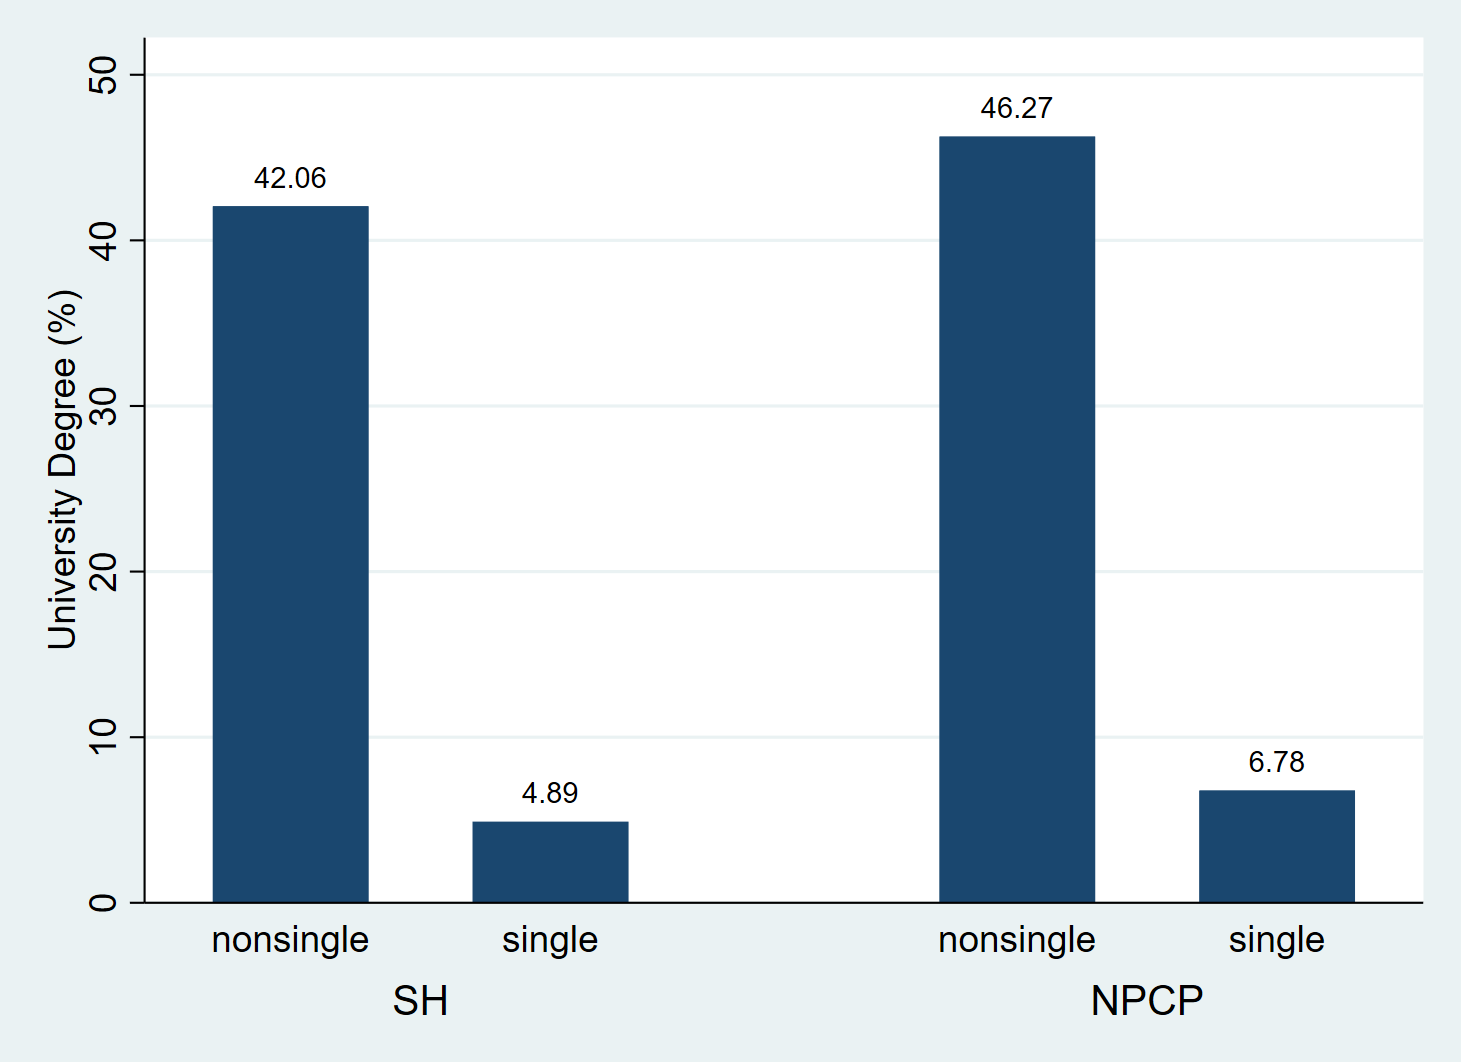
\includegraphics[width=0.76\textwidth, height=0.76\textheight]{"C:/Users/Administrator/Desktop/LaborTopicTermPaper/pic/university_sp.png"}
    \end{figure}

\end{frame}


\begin{frame} % 2-4.
\frametitle{Concerned Variable}
\framesubtitle{Outcome Variable (2): Master Degree}

    \begin{figure}
        \centering
        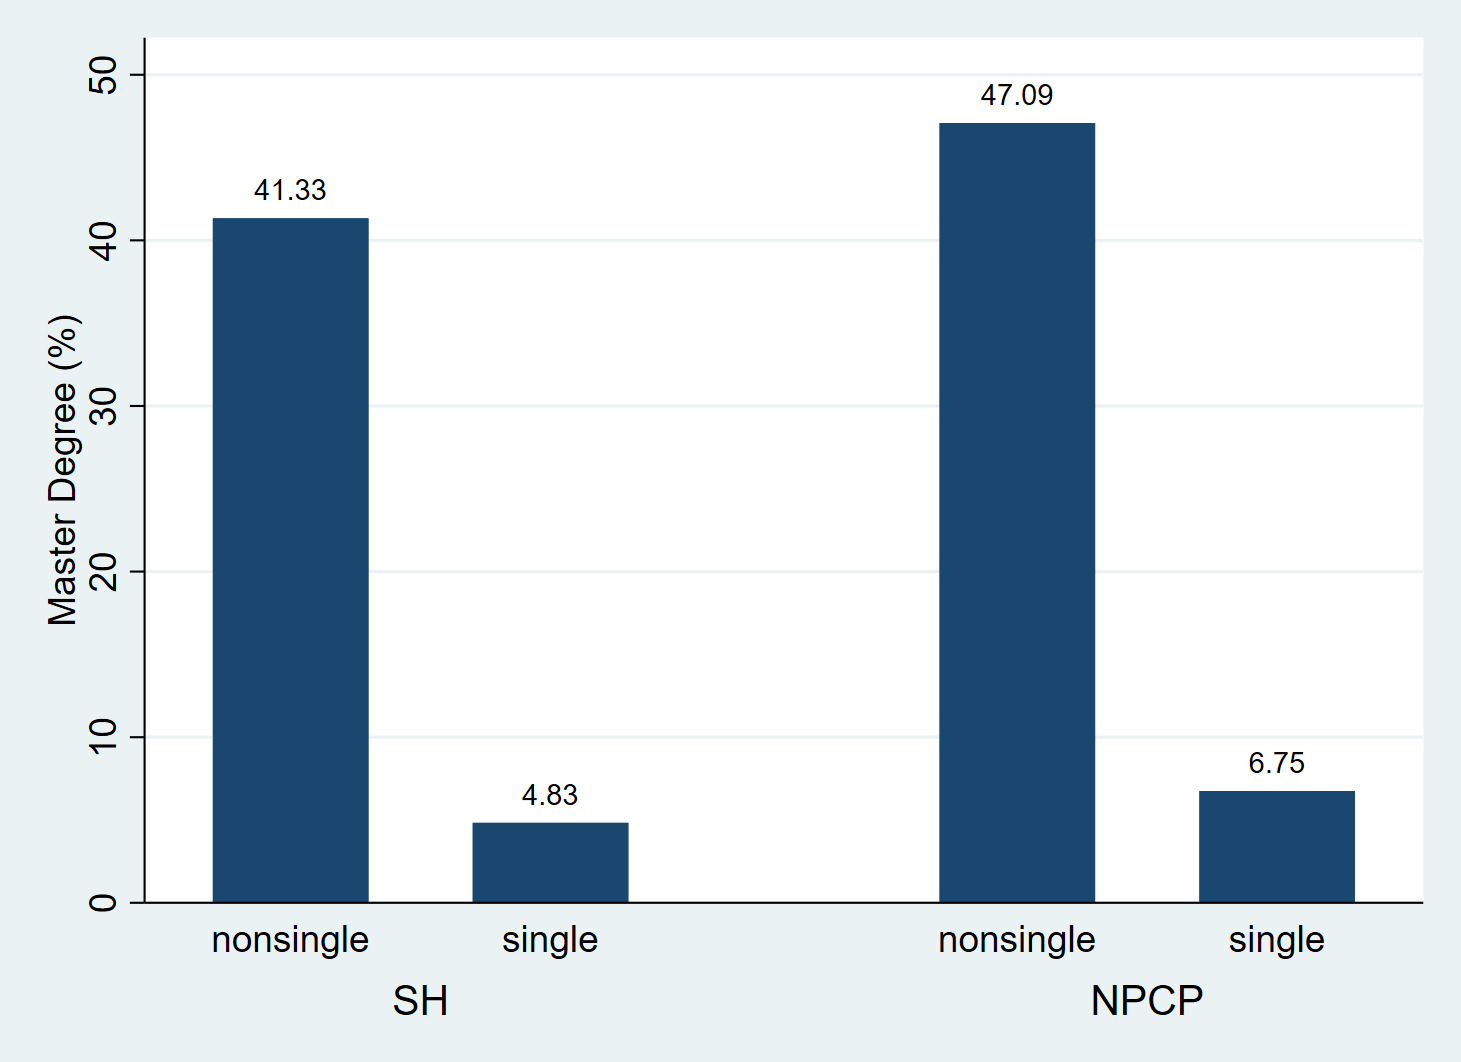
\includegraphics[width=0.76\textwidth, height=0.76\textheight]{"C:/Users/Administrator/Desktop/LaborTopicTermPaper/pic/master_sp.png"}
    \end{figure}

\end{frame}


\begin{frame} % 2-5.
\frametitle{Concerned Variable}
\framesubtitle{Outcome Variable (3): Public University}

    \begin{figure}
        \centering
        \label{Fig.sub.1}
        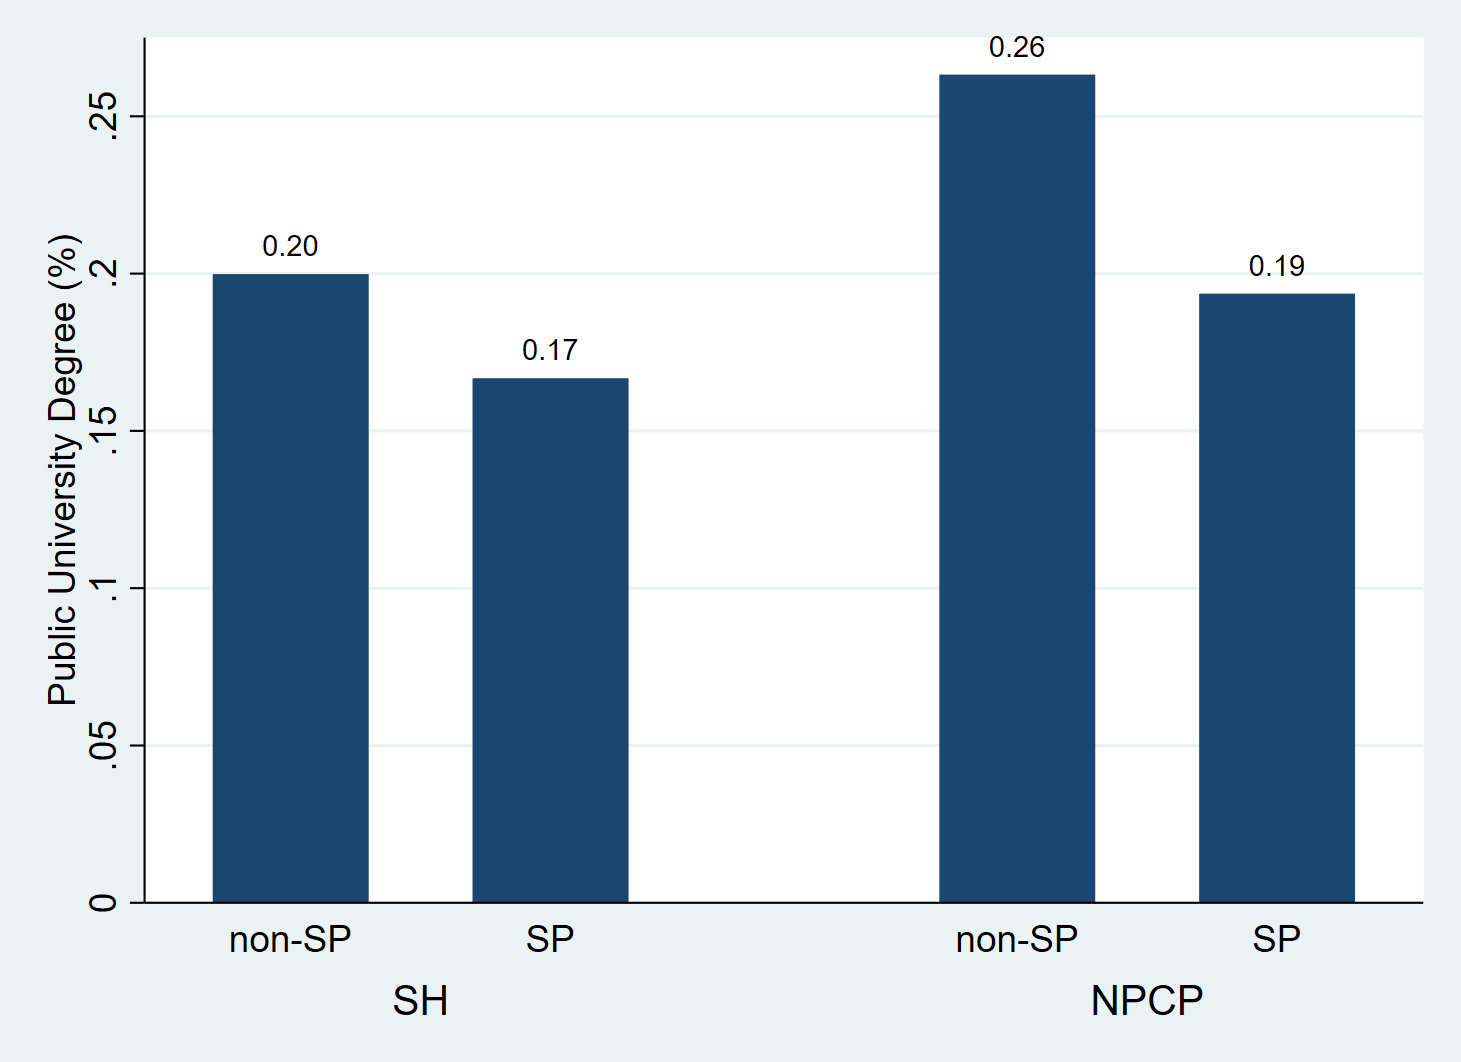
\includegraphics[width=0.76\textwidth, height=0.76\textheight]{"C:/Users/Administrator/Desktop/LaborTopicTermPaper/pic/public_sp.png"}
    \end{figure}

\end{frame}


\begin{frame} % 2-6.
\frametitle{Concerned Variable}
\framesubtitle{How to pick up potential confounders?}

    \begin{itemize}
        \item To perform PDS analysis, We pick an abundance of covariates, including 
            \begin{itemize}
                \item student's background information
                \begin{itemize}
                    \item gender, living area, private/public school, general/vocational school
                \end{itemize}        
                \item parent's education
                \item each teacher's evalutaion 
                \item etc. 
            \end{itemize}
        \item It's important to not include \textbf{bad control} in the model, hence we use very few covariates in parent's dataset
    \end{itemize}

\end{frame}


\begin{frame} % 3.
\frametitle{Empirical Specification}
\framesubtitle{Post-Double Selection}

    \begin{itemize}
        \item With PDS, we can detect the confounders in roughly \textbf{80 selected covariates} and identify the causal relationship
        \[
        Y_i = \beta_0 + \beta_1 \textit{SP}_i + \bigcup_{j \in A \cup B} \pi_j W_i^j + \epsilon_i
        \]
        where $A,B$ are the Lasso-selected covariates at step 1 \& 2 in PDS.
    \end{itemize}

\end{frame}
    

\begin{frame}[shrink=38] % 4-1.
\frametitle{Preliminary Result}
\framesubtitle{Outcome Variable (1): University Degree}

\centering
\begin{tabular}{l*{6}c}
    \toprule
    &\multicolumn{3}{c}{SH} &\multicolumn{3}{c}{CP/NP} \\
    \cmidrule(l){2-4}\cmidrule(l){5-7}
    &\multicolumn{1}{c}{(1)}&\multicolumn{1}{c}{(2)}&\multicolumn{1}{c}{(3)}&\multicolumn{1}{c}{(4)}&\multicolumn{1}{c}{(5)}&\multicolumn{1}{c}{(6)} \\
    &\multicolumn{1}{c}{University}&\multicolumn{1}{c}{University}&\multicolumn{1}{c}{University}&\multicolumn{1}{c}{University}&\multicolumn{1}{c}{University}&\multicolumn{1}{c}{University} \\
    \midrule
    sp & -0.0799\sym{***}& -0.0318\sym{***}& -0.0136     & -0.0989\sym{***}& -0.0230\sym{**} & -0.0264\sym{**} \\
    & (0.000)     & (0.008)     & (0.402)     & (0.000)     & (0.022)     & (0.041)     \\
    [1em]
    female  &   & 0.00945     &   &   &    0.000753     &   \\
    &   & (0.180)     &   &   & (0.902)     &   \\
    [1em]
    hs\_private  &   & -0.0762\sym{***}& -0.0386\sym{***}&   & -0.0896\sym{***}&   \\
    &   & (0.000)     & (0.000)     &   & (0.000)     &   \\
    [1em]
    hs\_urban    &   &  0.0711\sym{***}&   &   &  0.0294\sym{***}&  0.0124     \\
    &   & (0.000)     &   &   & (0.000)     & (0.159)     \\
    [1em]
    general\_high&   &   0.556\sym{***}&   0.514\sym{***}&   &   0.635\sym{***}&   \\
    &   & (0.000)     & (0.000)     &   & (0.000)     &   \\
    [1em]
    paedu   &   &   0.101\sym{***}&  0.0739\sym{***}&   &  0.0829\sym{***}&  0.0330\sym{***}\\
    &   & (0.000)     & (0.000)     &   & (0.000)     & (0.000)     \\
    [1em]
    PDS\_control  &   &  &  Yes    &  &    &  Yes \\
    \hline
    \(N\)   &   11132     &   11050     &    5230     &   12576     &   12386     &    5766     \\
    \bottomrule
    \multicolumn{7}{l}{\footnotesize \textit{p}-values in parentheses} \\
    \multicolumn{7}{l}{\footnotesize \sym{*} \(p<0.10\), \sym{**} \(p<0.05\), \sym{***} \(p<0.01\)} \\
\end{tabular}

\end{frame}


\begin{frame}[shrink=38] % 4-2.
\frametitle{Preliminary Result}
\framesubtitle{Outcome Variable (2): Master Degree}

\centering
\begin{tabular}{l*{6}c}
    \toprule
    &\multicolumn{3}{c}{SH} &\multicolumn{3}{c}{CP/NP} \\
    \cmidrule(l){2-4}\cmidrule(l){5-7}
    &\multicolumn{1}{c}{(1)}&\multicolumn{1}{c}{(2)}&\multicolumn{1}{c}{(3)}&\multicolumn{1}{c}{(4)}&\multicolumn{1}{c}{(5)}&\multicolumn{1}{c}{(6)} \\
    &\multicolumn{1}{c}{University}&\multicolumn{1}{c}{University}&\multicolumn{1}{c}{University}&\multicolumn{1}{c}{University}&\multicolumn{1}{c}{University}&\multicolumn{1}{c}{University} \\
    \midrule
    sp          &     -0.0753\sym{***}&     -0.0481\sym{***}&     -0.0405\sym{**} &     -0.0714\sym{***}&     -0.0404\sym{***}&     -0.0465\sym{**} \\
                &     (0.000)         &     (0.000)         &     (0.024)         &     (0.000)         &     (0.000)         &     (0.015)         \\
    [1em]
    female      &                     &     -0.0981\sym{***}&     -0.0597\sym{***}&                     &      -0.101\sym{***}&     -0.0558\sym{***}\\
                &                     &     (0.000)         &     (0.000)         &                     &     (0.000)         &     (0.000)         \\
    [1em]
    hs\_private  &                     &     -0.0763\sym{***}&                     &                     &     -0.0555\sym{***}&                     \\
                &                     &     (0.000)         &                     &                     &     (0.000)         &                     \\
    [1em]
    hs\_urban    &                     &      0.0536\sym{***}&                     &                     &      0.0497\sym{***}&      0.0570\sym{***}\\
                &                     &     (0.000)         &                     &                     &     (0.000)         &     (0.000)         \\
    [1em]
    general\_high&                     &       0.204\sym{***}&       0.156\sym{***}&                     &       0.167\sym{***}&                     \\
                &                     &     (0.000)         &     (0.000)         &                     &     (0.000)         &                     \\
    [1em]
    paedu       &                     &       0.156\sym{***}&       0.129\sym{***}&                     &       0.105\sym{***}&      0.0813\sym{***}\\
                &                     &     (0.000)         &     (0.000)         &                     &     (0.000)         &     (0.000)         \\
    [1em]
    PDS\_control  &                     &                    &      Yes             &                   &                 &      Yes \\
                
    \hline
    \(N\)       &       10438         &       10362         &        4848         &       12173         &       11986         &        5600         \\
    \bottomrule
    \multicolumn{7}{l}{\footnotesize \textit{p}-values in parentheses} \\
    \multicolumn{7}{l}{\footnotesize \sym{*} \(p<0.10\), \sym{**} \(p<0.05\), \sym{***} \(p<0.01\)} \\
\end{tabular}

\end{frame}


\begin{frame}[shrink=38] % 4-3.
\frametitle{Preliminary Result}
\framesubtitle{Outcome Variable (3): Public University}

\centering
\begin{tabular}{l*{6}c}
    \toprule
    &\multicolumn{3}{c}{SH} &\multicolumn{3}{c}{CP/NP} \\
    \cmidrule(l){2-4}\cmidrule(l){5-7}
    &\multicolumn{1}{c}{(1)}&\multicolumn{1}{c}{(2)}&\multicolumn{1}{c}{(3)}&\multicolumn{1}{c}{(4)}&\multicolumn{1}{c}{(5)}&\multicolumn{1}{c}{(6)} \\
    &\multicolumn{1}{c}{University}&\multicolumn{1}{c}{University}&\multicolumn{1}{c}{University}&\multicolumn{1}{c}{University}&\multicolumn{1}{c}{University}&\multicolumn{1}{c}{University} \\
    \midrule
    sp          &     -0.0331\sym{***}&    -0.00861         &     0.01000         &     -0.0696\sym{***}&     -0.0374\sym{***}&     -0.0443\sym{**} \\
                &     (0.006)         &     (0.450)         &     (0.553)         &     (0.000)         &     (0.001)         &     (0.020)         \\
    [1em]
    female      &                     &    -0.00220         &                     &                     &     -0.0278\sym{***}&                     \\
                &                     &     (0.757)         &                     &                     &     (0.000)         &                     \\
    [1em]
    hs\_private  &                     &      -0.103\sym{***}&     -0.0675\sym{***}&                     &      -0.120\sym{***}&     -0.0860\sym{***}\\
                &                     &     (0.000)         &     (0.000)         &                     &     (0.000)         &     (0.000)         \\
    [1em]
    hs\_urban    &                     &      0.0751\sym{***}&                     &                     &      0.0841\sym{***}&      0.0968\sym{***}\\
                &                     &     (0.000)         &                     &                     &     (0.000)         &     (0.000)         \\
    [1em]
    general\_high&                     &       0.229\sym{***}&       0.184\sym{***}&                     &       0.275\sym{***}&                     \\
                &                     &     (0.000)         &     (0.000)         &                     &     (0.000)         &                     \\
    [1em]
    paedu       &                     &       0.118\sym{***}&      0.0978\sym{***}&                     &       0.108\sym{***}&      0.0641\sym{***}\\
                &                     &     (0.000)         &     (0.000)         &                     &     (0.000)         &     (0.000)         \\
    [1em]
    PDS\_control  &                     &                    &      Yes             &                   &                 &      Yes \\
    \hline
    \(N\)       &       10577         &       10503         &        5027         &       11518         &       11353         &        5576         \\
    \bottomrule
    \multicolumn{7}{l}{\footnotesize \textit{p}-values in parentheses} \\
    \multicolumn{7}{l}{\footnotesize \sym{*} \(p<0.10\), \sym{**} \(p<0.05\), \sym{***} \(p<0.01\)} \\
\end{tabular}

\end{frame}


\begin{frame} % 5-1.
\frametitle{Concluding and Future Prospect}
\framesubtitle{What do PDS tells us?}

    \begin{itemize}
        \item There're many unexpected variables PDS selected, like
        \begin{itemize}
        \item \textsl{"How many years had the teacher taught in school?"}
        \item \textit{"What's the score/performance for this class?"}
        \item \textit{"Does the teacher hold extra class in the weekend?"}
        \item \textit{"How many student's parents the teacher had met with in this semester?"}
        \end{itemize}
        \item PDS surely help us reduce the OVB in a convenient way
        \begin{itemize}
            \item however, missing data problem comes with dimension, leading to significantly decreasing number of samples
        \end{itemize}
    \end{itemize}

\end{frame}
    

\begin{frame} % 5-2.
\frametitle{Concluding and Future Prospect}
\framesubtitle{What and How can we dive deeper?}

    \begin{itemize}
        \item Focus on the difference between two groups (SH vs. CPNP)
        \begin{itemize}
        \item high education reform in 2000s
        \end{itemize}
        \item Explain the negative effect (Mediation Analysis)
        \begin{itemize}
        \item accompanying time
        \item economic condition
        \end{itemize}
    \end{itemize}

\end{frame}


\end{document}
